\documentclass[DM,lsstdraft,authoryear,toc]{lsstdoc}
\input{meta}

% Package imports go here.
\usepackage{hyperref}
% Local commands go here.

%If you want glossaries
%\input{aglossary.tex}
%\makeglossaries

\begin{document}
\title{An introduction to Analysis Tools}

% This can write metadata into the PDF.
% Update keywords and author information as necessary.
\hypersetup{
    pdftitle={An introduction to Analysis Tools},
    pdfauthor={Sophie Reed},
    pdfkeywords={}
}

% Optional subtitle
% \setDocSubtitle{A subtitle}

\input{authors}

\setDocRef{DMTN-314}
\setDocUpstreamLocation{\url{https://github.com/lsst-dm/dmtn-314}}

\date{\vcsDate}

% Optional: name of the document's curator
% \setDocCurator{The Curator of this Document}

\setDocAbstract{%
Analysis Tools is a package designed for validation and verification of the
pipelines and the data they produce.It runs as part of the standard process and
produces a suite of metrics and plots that can be used to test the quality of
the outputs.  The Analysis Tools package is extensively documented, including
worked examples and plots, on the pipelines documentation page. Which can be
found here:
\url{https://pipelines.lsst.io/modules/lsst.analysis.tools/index.html} }

% Change history defined here.
% Order: oldest first.
% Fields: VERSION, DATE, DESCRIPTION, OWNER NAME.
% See LPM-51 for version number policy.
\setDocChangeRecord{%
  \addtohist{1}{YYYY-MM-DD}{Unreleased.}{First Last}
}


\begin{document}

% Create the title page.
\maketitle
% Frequently for a technote we do not want a title page  uncomment this to remove the title page and changelog.
% use \mkshorttitle to remove the extra pages

% ADD CONTENT HERE
% You can also use the \input command to include several content files.
Analysis Tools is a QA framework designed to perform routine validation and
verification upon the Rubin Science Pipelines and the data that they produce.
The available metrics and plots, along with the pipelines that produce them are
detailed on the main documentaion page
\url{https://pipelines.lsst.io/modules/lsst.analysis.tools/index.html}, which is kept
up to date as more tooling is added. These documentation pages also include a
Getting Started Guide which details how to add new plots and metrics.

The backbone of an Analysis Tools pipeline is the atools, these calculate
metrics and make plots.  The atools are designed to make calculation and
analysis on large datasets reproducule and rapid. For example they
automatically specify which columns (for example) should be read in from the
given dataset, helping to reduce the memory load when large data sets are used.
They are flexible and reproducible, the same atool can be run on different
datasets, for example pre and post calibration. Everything needed to reproduce
the atool exactly is saved with the result so that they can rerun and
investigated further when data issues are found. An atool is made up of various
components that can be assembled to fit the individual needs of the given
metric/plot.  They are predominantley made up of selector actions, calculate
actions and then plotting/metric actions that save the final output, and can
dispatch it to various pieces of monitoring interface.

\textbf{Selectors}\newline
The atool works out the required data from the specified selectors. We
encourage people to use the predefined selectors for uniformity across the
metrics but they are easy to implement if a different data selection. Selectors
return a mask specifying a subset of the initial data, this subset might be
defined through a signal to noise cut or through specific flag requirements.
There are predefinied selectors that use the flag cuts that DM recommends for a
clean set of data. These selectors are defined for both coadd and visit level
catalogues. This allows reproducibility of the standard plots that DM makes as
part of the standard processing. Selectors that perform standard selections,
such as S/N are fully configurable allowing the different components of the
final selection to be reused between atools.

\textbf{Calculate Actions}\newline
These actions are the main work horse of the atool, they take in the
subselected data produced by the combination of selectors used and then perform
the calculations required to generate the data for the requested metrics and
plots. For example to look at the difference between the PSF and CModel
magnitudes for stars with a S/N greater than 100, one would first apply a star
selector and a S/N selector to subselect the data. From this sub selected data
the magnitudes can be calculated from the fluxes by the appropriate
calculate action and subtracted from each other to give the values for all of
the data points.

\textbf{Metric and Plot Actions}\newline
Now that the data has been wrangled it can be passed to the plotting and metric
actions. There are a variety of plot types predefined and examples of these can
be found on the documentation pages linked above. Continuing the previous example
one might wish to check for spatial distributions within the PSF -
CModel difference which might indicate a spatial issue with the calculation of
the PSF. For this purpose the sky plot can be used, shown below in Figure
\ref{fig:skyPlot}. If a summary of the differences for the whole dataset is wanted
then the scatter plot might be more appropriate, Figure \ref{fig:scatterPlot},
a simplified version of this can also be made for publications and
presentations, Figure \ref{fig:scatterPlotPub}. Metrics from this data, for example
the median and sigma MAD of the magnitude difference can be calculated and
saved. As part of the standard processing these values are automatically
calculated and dispatched to our monitoring software. 

\begin{figure}
\centering
        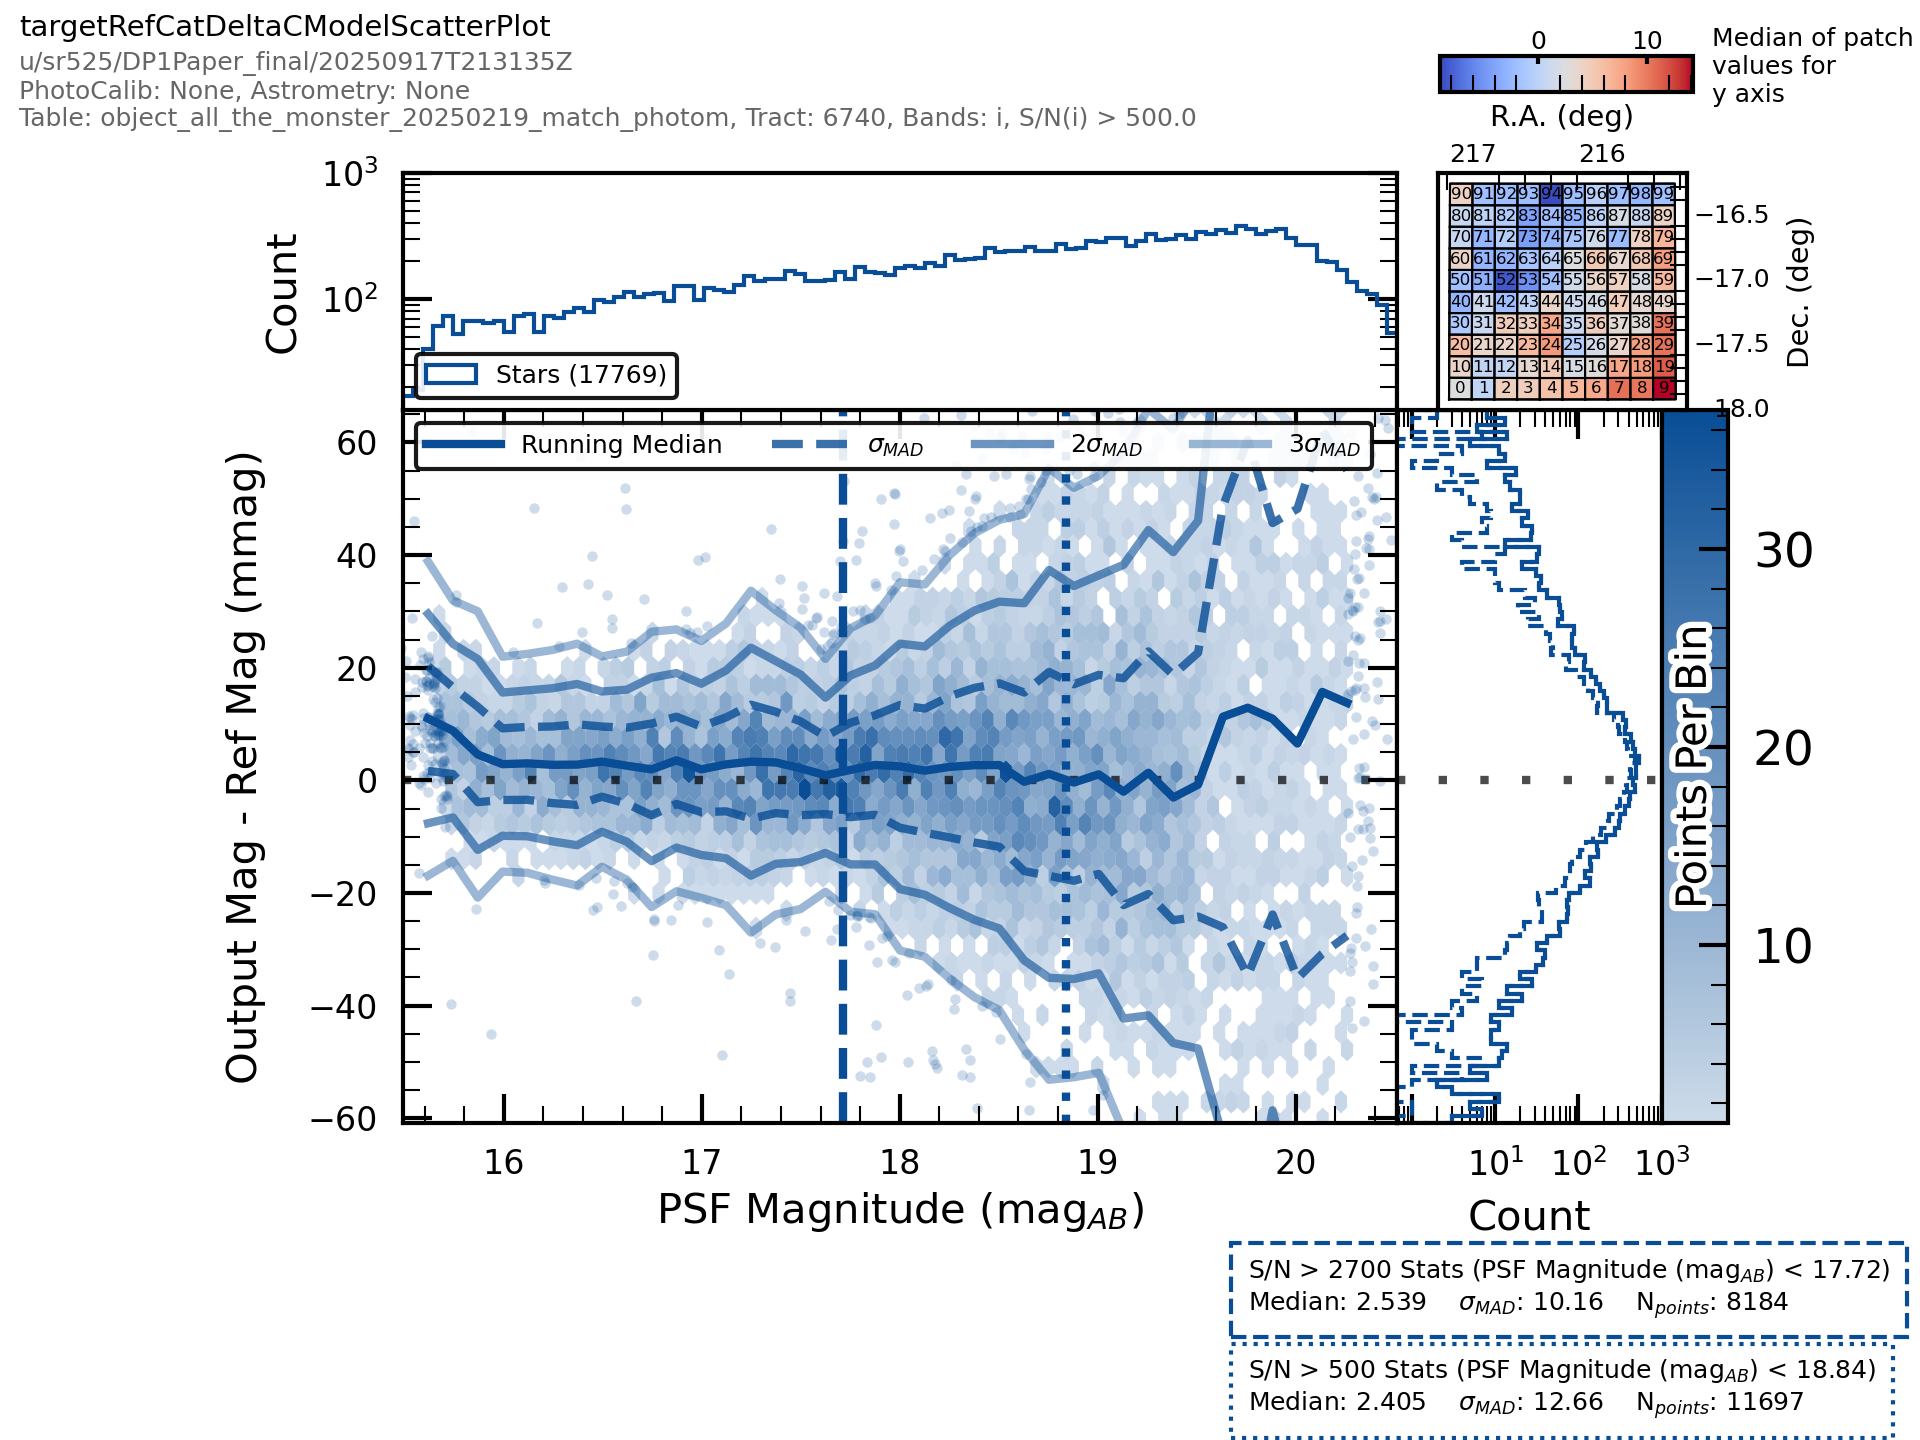
\includegraphics{scatterPlot.png}
    \caption{A plot showing the differences in magnitude between the magnitude calculated by the Rubin Sciene Pipelines and those for the same objects from Pan-STARRS. The data from each survey is first matched by a precursor task in analysis tools. The combined catalogue is then written out and used by the atools to calculate various metrics and plots.}
    \label{fig:scatterPlot}
\end{figure}

\begin{figure}
\centering
        \includegraphics{scatterPlotPub.png}
    \caption{A plot showing the differences in magnitude between the magnitude calculated by the Rubin Sciene Pipelines and those for the same objects from Pan-STARRS. The data from each survey is first matched by a precursor task in analysis tools. The combined catalogue is then written out and used by the atools to calculate various metrics and plots.}
    \label{fig:scatterPlotPub}
\end{figure}

\begin{figure}
\centering
        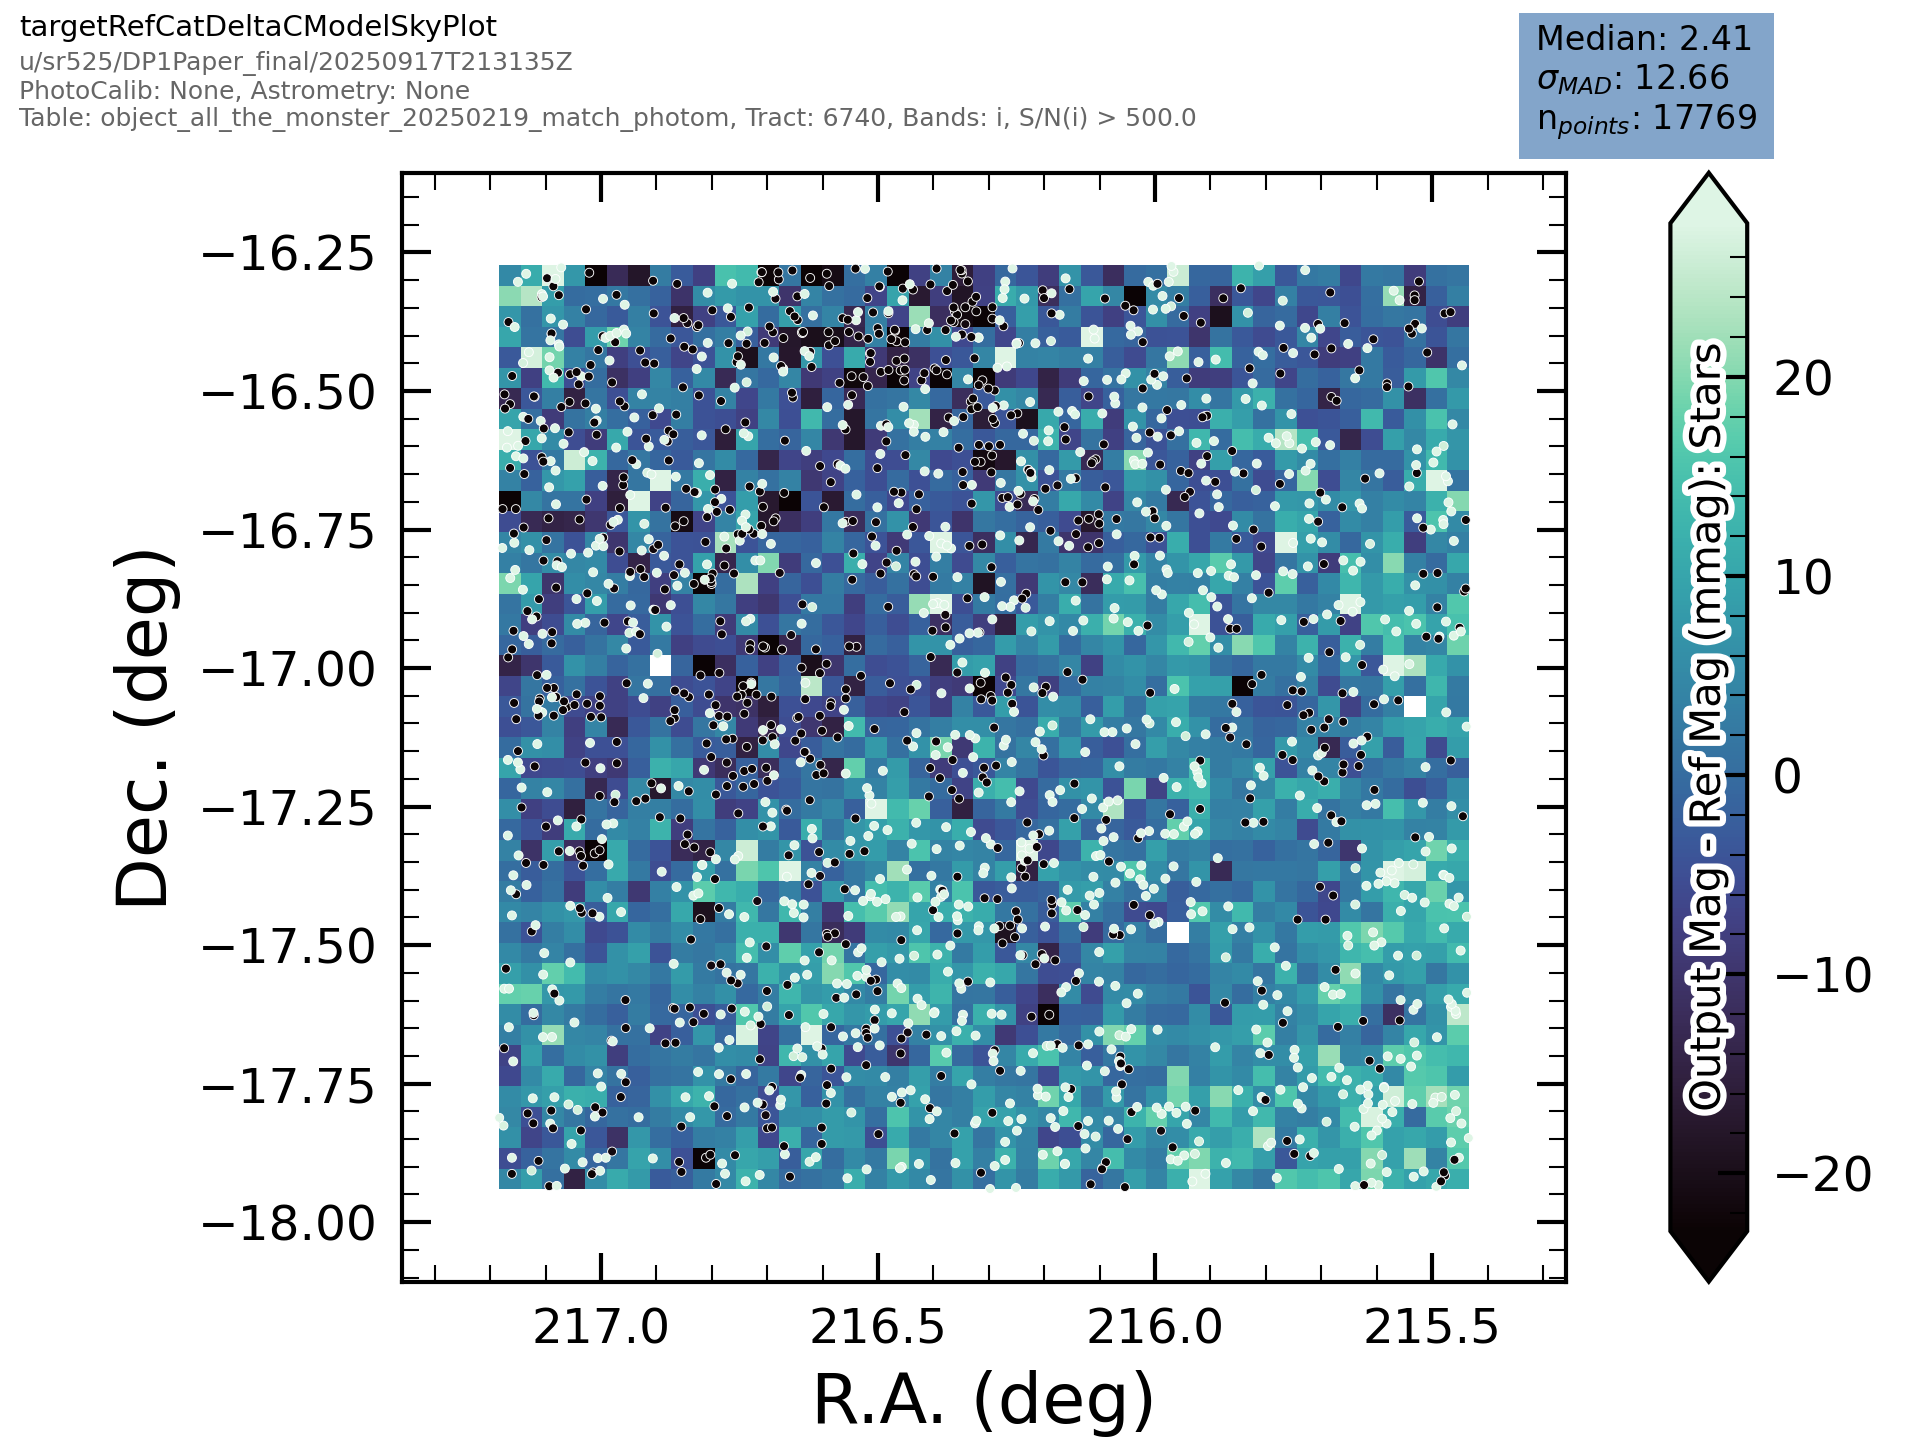
\includegraphics{skyPlot.png}
    \caption{A plot showing the differences in magnitude between the magnitude calculated by the Rubin Sciene Pipelines and those for the same objects from Pan-STARRS. The data from each survey is first matched by a precursor task in analysis tools. The combined catalogue is then written out and used by the atools to calculate various metrics and plots.}
    \label{fig:skyPlot}
\end{figure}



More complicated atools such as those using matched datasets, might require a
precursor task to wrangle the initial data into a form that the atools can
efficently access, this intermediate product can be saved to allow easier
debugging if a problem is found.


\appendix
% Include all the relevant bib files.
% https://lsst-texmf.lsst.io/lsstdoc.html#bibliographies
\section{References} \label{sec:bib}
\renewcommand{\refname}{} % Suppress default Bibliography section
\bibliography{local,lsst,lsst-dm,refs_ads,refs,books}

% Make sure lsst-texmf/bin/generateAcronyms.py is in your path
\section{Acronyms} \label{sec:acronyms}
\addtocounter{table}{-1}
\begin{longtable}{p{0.145\textwidth}p{0.8\textwidth}}\hline
\textbf{Acronym} & \textbf{Description}  \\\hline

DM & Data Management \\\hline
DMTN & DM Technical Note \\\hline
PSF & Point Spread Function \\\hline
Pan-STARRS & Panoramic Survey Telescope and Rapid Response System \\\hline
QA & Quality Assurance \\\hline
\end{longtable}

% If you want glossary uncomment below -- comment out the two lines above
%\printglossaries





\end{document}
